\documentclass{article}

\usepackage[fleqn]{amsmath}
\usepackage{amssymb}
\usepackage{hyperref}
\usepackage{url}
\usepackage{graphicx}
\usepackage{geometry}
\usepackage{babel}
\usepackage{enumitem}
\usepackage{parskip}
\usepackage{chemfig}
\usepackage{pdfpages}
\usepackage{xcolor}
\usepackage{tikz}
\usepackage{fancybox}
\usepackage{makecell}
\usepackage{pgfplots}
\usepackage{soul}
\usepackage{ulem}
\usepackage{wrapfig}
\usepackage{subcaption}
\usepackage[T1]{fontenc}
\usepackage{pgfplots}
\usetikzlibrary{arrows}
\usetikzlibrary{decorations.pathreplacing}
\pgfplotsset{compat=1.17}

\geometry{
    a4paper,
    total={170mm, 257mm},
    left=20mm,
    top=20mm
}

\hypersetup{
    colorlinks=true,
    linkcolor=black,
    urlcolor=blue,
    pdftitle={Math refreshing course}
}

\newcommand{\figbox}[1]{ 
    \begin{figure*}[ht!]        
        \begin{center}            
            \fbox{#1}        
        \end{center}    
    \end{figure*}
}

% === TEXT ===
\title{\textbf{Maths refreshing course \\ HSLU, Semester 1}}
\author{Matteo Frongillo}

\begin{document}

\maketitle
\tableofcontents
\pagebreak

\part{Lesson 1}

\section{Numerical sets}
\begin{itemize}
    \item $\mathbb{N} := \text{Natural numbers (including 0)}$
    \item $\mathbb{Z} := \text{Integer numbers}$
    \item $\mathbb{Q} := \text{Rational numbers}$
    \item $\mathbb{R} := \text{Real numbers}$
\end{itemize}

\underline{Notation}: The ``$^*$'' symbol means that the set does not include 0.

We have that: 
\[
    \mathbb{N} \subset  \mathbb{Z} \subset \mathbb{Q} \subset \mathbb{R} \subset \mathbb{C} 
\]

\section{Prime numbers}
A prime number is a number \( n \in \mathbb{N} \setminus \{0,1\} \) such that, for every divisor \( d \in \mathbb{N} \), if \( d \mid n \), then \( d = 1 \) or \( d = n \).
\figbox{$n \in \mathbb{N} \setminus \{0,1\} \text{ is prime} \iff \forall d \in \mathbb{N}, (d \mid n) \Rightarrow (d = 1 \ \text{or} \ d = n)$}

\section{Positive powers}
Let $a \in \mathbb{R}, n \in \mathbb{R}^*$ and ${a} \subset \mathbb{R}$, then

\figbox{$
    a^{1} := a \quad | \quad
    a^n = \underbrace{a \cdot a \cdot ... \cdot a}_{n \text{ times}}$
}

\subsection{Property 1}
Let $a, b \in \mathbb{R},\ n,m \in \mathbb{N}$, then \\
\figbox{$a^n \cdot a^m = a^{n+m}$}

\subsection{Property 2}
Let $a,b \in \mathbb{R},\ n \in \mathbb{N}$, then \\
\figbox{$(a \cdot b)^n = a^n \cdot b^n$}

\underline{Notation}: The power $a^n$, $a$ is the base and $n$ is the exponent.

\subsection{Property 3}
Let $a \in \mathbb{R},\ m,n \in \mathbb{N}^*$, then \\
\figbox{$(a^n)^m = a^{n \cdot m}$, which is $\neq a^{(n^m)}$}

\newpage
\section{Fractions}
\underline{Notation 1}: $a \cdot b = a \times b = ab$ \quad | \quad $\frac{a}{b} = a \div b = a : b$

\underline{Notation 2}: ``$a$'' is called numerator, ``$b$'' is called denominator.

\underline{Notation 3}: $\frac{a}{b},\ a,b \in \mathbb{R},\ b \neq 0$

\subsection{Property 1}
Let $a, b \in \mathbb{R}^*$ and $c, d \in \mathbb{R}$, then\\
\figbox{\large $\frac{a}{b} \cdot \frac{c}{d} = \frac{a \cdot c}{b \cdot d}$}

\subsection{Property 2}
Let $a, b \in \mathbb{R}^*$ and $c, d \in \mathbb{R}$, then\\
\figbox{\large $\frac{a}{b} \div \frac{c}{d} = \frac{a}{b} \cdot \frac{d}{c}$}

\subsection{Property 3}
Let $a, b \in \mathbb{R}^*$ and $c, d \in \mathbb{R}$, then\\
\figbox{\large $\frac{a}{b} \pm \frac{c}{d} = \frac{a \cdot d \pm c \cdot b}{b \cdot d}$}

\section{Negative powers}
\subsection{Definition}
\figbox{$\forall a \in \mathbb{R}^*$; \; $a^{-1} := \frac{1}{a} $}

\subsection{Property 4}
Let $\forall n \in \mathbb{N},\ \forall a \in \mathbb{R}$, then\\
\figbox{$a^{-n} = \left(\frac{1}{a}\right)^n$}

This property implies that $\forall z \in \mathbb{Z},\ \forall a \in \mathbb{R},\ z \neq 0$\\
We can compute $a^z$

\subsection{Property 5}
Let $\forall a \in \mathbb{R},\ a \neq 0,\ \forall n,m \in \mathbb{Z}$, then\\
\figbox{$\frac{a^n}{a^m} = a^{n-m}$}

\newpage
\underline{Consequences}:
\begin{enumerate}
    \item Properties 1, 2 and 3 also hold for integer exponents:
        \begin{itemize}
            \item $\forall a \in \mathbb{R},\ \forall n,m \in \mathbb{Z} \Rightarrow a^n \cdot a^m = a^{n+m}$
            \item $\forall b \in \mathbb{R},\ (a \cdot b)^n = a^n \cdot b^n$
            \item $(a^n)^m = a^{n \cdot m}$
        \end{itemize}  
    \item $\forall a \in \mathbb{R}^*,\ a^0 = a^{1-1} = \frac{a^1}{a^1} = 1 \Rightarrow a^0 = 1$
\end{enumerate}

\section{Fractions and percentages (and back)}
$\alpha \in \mathbb{R},\ n \% \text{ of } \alpha \Longleftrightarrow \frac{n}{100} \cdot \alpha$

\newpage
\part{Lesson 2}

\section{Symbols}
Let $a,b \in \mathbb{R}$, then
\begin{itemize}[label=--]
    \item $a=b \rightarrow$ equality;
    \item $a \neq b \rightarrow$ inequality ($a$ is not equal to $b$);
    \item $a<b \rightarrow$ less than (a is strictly less than b);
    \item $a\leq b \rightarrow$ less than or equal to ($a$ is less than or equal to $b$);
    \item $a>b \rightarrow$ greater than ($a$ is strictly greater than $b$);
    \item $a\geq b \rightarrow$ greater than or equal to ($a$ is greater than or equal to $b$).
\end{itemize}

\underline{Example}: $x \in \mathbb{R},\ x \geq 2 \rightarrow 2 \leq x < \infty$

\section{Brackets}
\begin{align*}
    &\left(\phantom{-}\right) \text{ \ Parenthesis (round brackets)}\\
    &\left[\phantom{-}\right] \text{ \, Square brackets}\\
    &\left\{\phantom{-}\right\} \text{ Braces}
\end{align*}

\section{Latin notations}
\begin{itemize}
    \item e.g. = for example;
    \item i.e. = that is / that implies;
    \item Q.E.D. ($\Box$)= quod erat demonstrandum (we finally prove it).
\end{itemize}

\section{The real line}
\vspace*{.5cm}
\begin{center}
    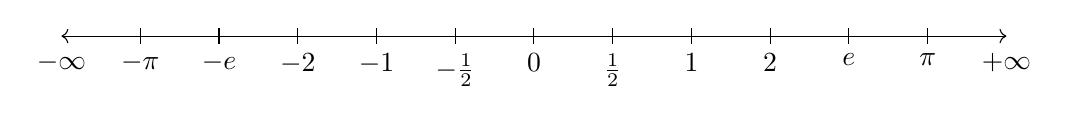
\begin{tikzpicture}
        \draw[->] (0,0) -- (6,0);
        \draw[<-] (-6,0) -- (0,0);
        
        \foreach \x/\label in {-5/{$-\pi$}, -4/{$-e$}, -3/{$-2$}, -2/{$-1$}, -1/{$-\frac{1}{2}$}, 0/{$0$}, 1/{$\frac{1}{2}$}, 2/{$1$}, 3/{$2$}, 4/{$e$}, 5/{$\pi$}} {
            \draw (\x,0.1) -- (\x,-0.1) node[below] {\label};
        }
        \node[below] at (-6,-0.1) {$-\infty$};
        \node[below] at (6,-0.1) {$+\infty$};
    \end{tikzpicture}
\end{center}

\subsection{Exercises}
1) $\forall a,b,x \in \mathbb{R},\ a \leq x \leq b$

\begin{center}
    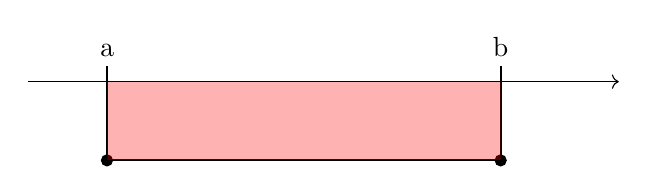
\begin{tikzpicture}
        %number line
        \draw[-] (-4,0) -- (3,0);
        \draw[thick] (-3,-0.2) -- (-3,0.2);
        \draw[thick] (2,-0.2) -- (2,0.2);
        
        %interval
        \draw[thick] (-3,-1) -- (2,-1);
        \draw[thick] (-3,0) -- (-3,-1);
        \draw[thick] (2,0) -- (2,-1);
        \filldraw[black] (-3,-1) circle (2pt);
        \filldraw[black] (2,-1) circle (2pt);
        
        %points
        \node[above] at (-3,0.2) {a};
        \node[above] at (2,0.2) {b};
        
        %arrow
        \draw[->] (3,0) -- (3.5,0);

        %area
        \filldraw [fill=red, draw=black, opacity=0.3] (-3,0) rectangle (2,-1);
    \end{tikzpicture}
\end{center}

2) $\forall x \in \mathbb{R},\ x \in\ ]-2,-1]\ \cup\ ] \frac{3}{2}, +\infty[$

\begin{center}
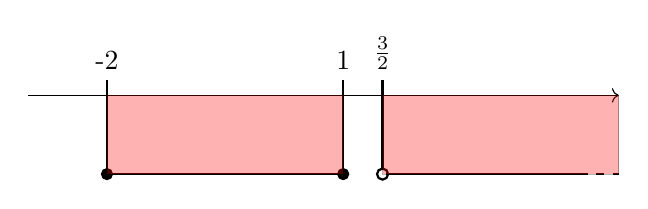
\begin{tikzpicture}
    %number line
    \draw[-] (-3,0) -- (4,0);
    \draw[thick] (-2,-1) -- (-2,0.2);
    \draw[thick] (1,-1) -- (1,0.2);
    \draw[thick] (1.5,-0.95) -- (1.5,0.2);
    
    %intervals
    \draw[thick] (-2,-1) -- (1,-1);
    \filldraw[black] (-2,-1) circle (2pt);
    \filldraw[black] (1,-1) circle (2pt);
    \draw[thick] (1.55,-1) -- (4,-1);
    \draw[thick, dashed] (4,-1) -- (4.5,-1);
    \draw[thick] (1.5,-1) circle (2pt);
    
    %points
    \node[above] at (-2,0.2) {-2};
    \node[above] at (1,0.2) {1};
    \node[above] at (1.5,0.2) {\(\frac{3}{2}\)};
    
    %arrow
    \draw[->] (4,0) -- (4.5,0);

    %area
    \filldraw [fill=red, draw=black, opacity=0.3] (-2,0) rectangle (1,-1);
    \filldraw [fill=red, draw=black, opacity=0.3] (1.5,0) rectangle (4.5,-1);
\end{tikzpicture}
\end{center}
\vspace*{.5cm}
\underline{Notation}: The union of two or more intervals where $x \in \mathbb{R}$
is denoted by the symbol $\cup$.

\newpage
\section{Properties of real numbers}
\subsection{Property 1 - Closure under ``$+$'' and ``$\cdot$''}
$\forall x,y \in \mathbb{R}\\
x+y \in \mathbb{R}\\    
x \cdot y \in \mathbb{R}$

\underline{Remark}: for $\forall x \in \mathbb{Z}$, closure does not hold for division.

\subsection{Property 2 - Commutativity}
$\forall x,y \in \mathbb{R}\\
x+y=y+x\\
x \cdot y=y \cdot x$

\underline{Remark}: commutativity does not hold for divisions and
subtractions.

\subsection{Property 3 - Associative}
$\forall x,y,z \in \mathbb{R}\\
x+(y+z) = (x+y)+z\\
x \cdot (y\cdot z)=(x\cdot y)\cdot z$

\underline{Remark}: associativity does not hold for divisions and
subtractions.

\subsection{Property 4 - Distributive}
$\forall x,y,z \in \mathbb{R}\\
x(y \pm z)=xy \pm xz$

\subsection{Property 5 - Identity}
$\forall x \in \mathbb{R}$
\begin{enumerate}[label=\alph*)]
    \item $0+x=x$
    \item $1 \cdot x=x$
\end{enumerate}

\underline{Remark}: $\forall x \in \mathbb{R},\ x \cdot 0=0$ is
\underline{not} an identity property.

\subsection{Property 6 - Inverses and opposites}
$\forall x \in \mathbb{R}$
\begin{enumerate}[label=\alph*)]
    \item $x+(-x)=0$ (additive inverse)
    \item when $x \neq 0,\ x \cdot \frac{1}{x}=1$ (multiplicative inverse or opposite)
\end{enumerate}

\underline{Remark 1}: $\forall x \in \mathbb{N}$ does not exist either
inverse nor opposite.

\underline{Remark 2}: $\forall x \in \mathbb{Z}$ has inverses, but
not opposites.

\section{The order of operations}
\begin{enumerate}
    \item Perform all operations inside grouping symbols beginning with the innermost set:\\
        $\left(\phantom{-}\right)$ inside brackets operations;
    \item Perform all exponential operations as you come to them, moving left-to-right:\\
        $x^a$;
    \item Perform all multiplications and divisions as you come to them, moving left-to-right:\\
        ``$\cdot$'' and ``$\div$'';
    \item Perform all additions and subtractions as you come to them, moving left-to-right:\\
        ``$+$'' and ``$-$'';
    \item When the level of priority is the same (e.g. multiplications and divisions) solve them as you come to them.
\end{enumerate}

\section{Signed numbers}
A number is denoted as positive if it is directly preceded by a $+$ sign or no sign at all.\\
A number is denoted as negative if it is directly preceded by a $-$ sign.

$\forall x \in \mathbb{R}$
\[-(-x)=x\\
+(-x)=-x\\
+(+x)=x\\
-(+x)=-x\]

\section{Absolute value}
Let $x \in \mathbb{R}$, then

$|x|=$
$\begin{cases}
    x \qquad \text{if } x \geq 0\\
    -x \;\quad \text{if } x < 0
\end{cases}$

\subsection{Property}
$\forall x \in \mathbb{R}\\
|x|>0 \quad \text{if } y \neq 0\\
|x|=0 \quad \text{if } x=0$

\newpage
\part{Lesson 3}
\section{Polynomials}
\subsection{Terms and factors}
\subsubsection{Variables}
A variable is a letter or a symbol which can assume every any value.
\figbox{$\forall x \in \mathbb{R}$}\\
Most common variables are $a$, $b$, $x$, $y$.

When we have an equality $y=x+a$, $\forall x \in \mathbb{R}$, $x$ can assume
every value in the set of real numbers ($x$ is an indipendent variable), while $y$ scrictly depends on the
value that we decided to give to x. 

\underline{Notice}: we can write $y=x+a$ as $y-a=x$, changing which variable is
indipendent and which is the dependent.

\subsubsection{Sets}
... ...
\figbox{In the set $\forall x \in \left[a,b\right]$, $x$ can assume every number between $a \leq x \leq b$}

\subsection{Expressions, terms and factors}
\subsubsection{Expressions}
An expression is any formula containing numbers, variables, operations, and
brackets.
\figbox{$y=ax^2+bx\cdot c$}

\subsubsection{Terms}
A term is any part of the expression separated by ``$+$'' or ``$-$''.
\figbox{$y = \underbrace{ax^2}_{term} + \underbrace{bx \cdot c}_{term}$}

\subsubsection{Factors}
Each term can be splitted into several factors separated by a multiplication sign.
\figbox{$x \cdot y \cdot (a-b) \cdot 24 = x \cdot y \cdot (a-b) \cdot 2 \cdot 2 \cdot 2 \cdot 3$}

\underline{Notice}: the process to split a term into several factors is called ``factorization''.\\
\phantom{} \hspace{1cm} The goal of a factorization is to factorize an expression as much as we can.

\newpage
\section{--}











\end{document}

